\subsubsection{}
\label{sec:analysis:research:mobArch:ufeature}

По своей сути приложения состоят из набора функциональных возможностей. Обычно все эти возможности приложения реализованы в пределах одного модуля. Результатом такого подхода является тесная связанность разных модулей, введение неявных зависимостей, увеличение сложности поддержки и разработки новых функций. Паттерн \gls{mvvm} предназначен для организации пользовательского интерфейса приложения, однако часто приложение можно условно разбить на несколько независимых доменов --- обычно каждый такой домен называется микросервисом.

Микросервисы предоставляют минимальный, но необходимый для интеграции \gls{api}, скрывая детали реализации. Для примера в iOS клиенте чата можно выделить следующие домены:

\begin{itemize}
	\item сервисы для шифрования сообщений, общения с сервером, работой с базой;
	\item экраны списка контактов, настроек, списка диалогов и конкретного диалога.
\end{itemize}

В 2017 году компания SoundCloud представила своё видение организации микросервисной архитектуры в мобильных приложениях: \textbf{uFeatures}.

uFeatures --- архитектурный подход для стуктурирования iOS приложений, предоставляющий масштабируемость, оптимизацию времени сборки проетка и циклов тестирования, гарантирующий адоптацию хороших практик разработки в команде. Основной идеей подхода является разработка независимых возможностей приложения, которые взаимодействуют при помощи чётко обозначенного \gls{api}. \cite{soundcloud:ufeature}

Типичная uFeature представляет из себя отдельный проект с 4 схемами:

\begin{itemize}
	\item код и ресурсы;
	\item тесты;
	\item данные, которые используются в тестах и приложении-примере;
	\item приложение-пример.
\end{itemize}

На рисунке \ref{sec:analysis:research:mobArch:ufeature:featureDependencyDiagram} представлена связь схем одного модуля uFeature.

\begin{figure}[h]
  \centering
    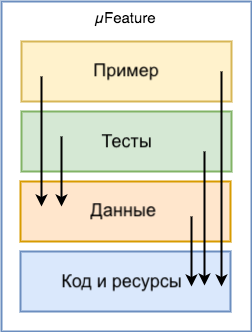
\includegraphics{inc/img/ufeature-diagram.png}
  \caption{Организация схем внутри модуля одной uFeature}
  \label{sec:analysis:research:mobArch:ufeature:featureDependencyDiagram}
\end{figure}

Автор подхода предлагает разделять все uFeature на два вида:

\begin{itemize}
	\item \emph{Foundation} --- основные строительные блоки, общие расширение пользовательского интерфейса, сервисы;
	\item \emph{Product} --- возможности, с которыми пользователь взаимодействует и видит на экране, например список диалогов;
\end{itemize}

